\testocapitolo{Dai, dai, dai!}
\chapter{Introduction}
\label{ch:introduction}

Al giorno d'oggi il Large Hadron Collider (LHC) è il collider di particelle più grande e potente al mondo che ha permesso, nel 2012, l'osservazione del bosone di Higgs, con massa attorno ai $125\,\GeV$~\cite{ATLAS:2012Higgs,CMS:2012Higgs}, completando il Modello Standard (SM). Con questa teoria è possibile descrivere tutti i fenomeni attualmente accessibili ai collider, e dopo quindici anni di attività LHC non ha trovato segnali di nuova fisica su un ordine di grandezza in energia attorno alla scala del $\TeV$.

Nonostante questo, restano ancora alcune domande aperte come l'asimmetria tra materia e antimateria, l'evidenza della materia oscura e le masse non nulle dei neutrini. Le risposte potrebbero trovarsi a scale di energia molto maggiori e pertanto richiedono uno strumento di esplorazione nuovo, più potente, che renda possibile la ricerca di fisica oltre lo SM (BSM) a energie sempre maggiori, e un programma che lo affianchi a LHC e al suo upgrade ad alta luminosità (HL-LHC).

Gli obiettivi di un simile strumento sono quattro~\cite{FCC:FSR-v1}:
\begin{itemize}
    \item mappare le proprietà del bosone di Higgs e dei bosoni di gauge elettrodeboli con precisioni di uno o più ordini di grandezza migliori delle attuali;
    \item condurre una campagna completa di misure di precisione elettrodeboli, di QCD, di sapore, dell'Higgs e del quark top, sensibile a deviazioni minime dal SM e a scale di energia molto oltre la portata cinematica diretta;
    \item migliorare di ordini di grandezza la sensibilità a fenomeni rari a bassa energia, incluse particelle leggere debolmente accoppiate e candidati di materia oscura;
    \item estendere di almeno un ordine di grandezza la portata di scoperta diretta di nuove particelle alla frontiera in energia.
\end{itemize}
Questi richiedono alte luminosità integrate alle scale elettrodeboli e dell'Higgs, e energie del centro di massa partonico un ordine di grandezza sopra il $\TeV$. La combinazione di questi due requisiti è stata indicata dalla comunità europea come priorità, sia nell'aggiornamento del 2020 della Strategia Europea per la Fisica delle Particelle~\cite{ESPP:2020}, che nel successivo aggiornamento del 2026~\cite{ESPP:2026}. 

Nei successivi paragrafi verranno descritti lo stato attuale della ricerca a LHC (sezione~\ref{sec:lhc}), le previsioni per la prossima fase ad alta luminosità (HL-LHC, (sezione~\ref{sec:hllhc})) e il progetto per il Future Circular Collider (FCC, (sezione~\ref{sec:fcc})).


\section{LHC e HL-LHC}
\label{sec:lhc}

\subsection{Il Large Hadron Collider e il suo programma}
LHC consiste in un anello di circa $27\,\mathrm{km}$ di circonferenza in cui collidono fasci di protoni (e, per periodi dedicati, di ioni pesanti), con quattro esperimenti principali, tra cui i due rivelatori generici ATLAS e CMS \todo{cita LHC machine paper}. Dopo il Run~1 a $7$-$8\,\TeV$ (2010-2012), nel quale è stato osservato il bosone di Higgs, il Run~2 (2015-2018) ha raccolto una luminosità integrata di circa $140\,\mathrm{fb^{-1}}$, per esperimento, a $13\,\TeV$, mentre il Run~3, (2022-2026), ha operato a $13.6\,\TeV$ \todo{cita}. 
 
La massa del bosone di Higgs è $125.20\pm0.11\,\GeV$, oggi nota con una precisione di circa un per mille e compatibile con quanto previsto dal SM con il meccanismo di rottura spontanea della simmetria elettrodebole (EWSSB), che una volta nota la massa predice l'intera fenomenologia dell'Higgs senza parametri liberi~\cite{FCC:FSR-v1}. 
È però necessario misurare le proprità del bosone di Higgs con la massima precisione possibile, perché ci sono molte ragioni per credere che il meccanismo di EWSSB sia sensibile a nuova fisica e possa essere legato ad alcune domande ancora senza risposta, come l'origine della massa, lo schema osservato delle masse dei fermioni (la struttura dei coefficienti di Yukawa), il problema della naturalezza e l'origine dell'asimmetria tra materia e antimateria~\cite{FCC:FSR-v1}.
 
\subsection{Il programma ad alta luminosità}
\label{sec:hllhc}
Il passo successivo del programma di LHC è l'High-Luminosity LHC, il cui obiettivo è raccogliere circa $3000\,\mathrm{fb^{-1}}$ per ciascun esperimento, cioè dieci volte la luminosità integrata inizialmente prevista per LHC. Questo risultato si ottiene aumentando di un fattore circa cinque la luminosità di picco rispetto al progetto originale, raddoppiando la corrente dei fasci e operando in regime di \emph{luminosity levelling}~\cite{Rossi:HLLHC2019,Rossi:Courier}. Per raggiungerlo sono necessarie nuove tecnologie:
\begin{itemize}
    \item nuovi quadrupoli di focalizzazione finale (\emph{inner triplets}) basati su cavi superconduttori di niobio-stagno ($\mathrm{Nb_3Sn}$) con campo di picco vicino ai $12\,\mathrm{T}$~\cite{Rossi:HLLHC2019,Rossi:Courier};
    \item \emph{crab cavities} compatte, che ruotano i pacchetti di protoni per mantenere collisioni quasi frontali~\cite{Rossi:HLLHC2019,Rossi:Courier};
    \item alcuni dipoli da $11\,\mathrm{T}$ in $\mathrm{Nb_3Sn}$, e collegamenti superconduttori da $100\,\mathrm{kA}$~\cite{Rossi:HLLHC2019};
    \item gallerie tecniche di nuova costruzione, collegate al tunnel di LHC con $28$ pozzi verticali~\cite{CERN:LS3}.
\end{itemize}
Gli esperimenti ATLAS e CMS sostituiranno una gran parte dei loro rivelatori e dell'elettronica (aggiornamenti di \emph{Phase-2}) per sostenere le condizioni di alta luminosità~\cite{CERN:LS3}. Le stesse tecnologie di magneti ad alto campo sono inoltre un passaggio chiave verso un collider adronico di nuova generazione~\cite{Rossi:HLLHC2019}, e costituiscono uno dei legami tra HL-LHC e FCC.

\begin{figure}[H]
    \centering
    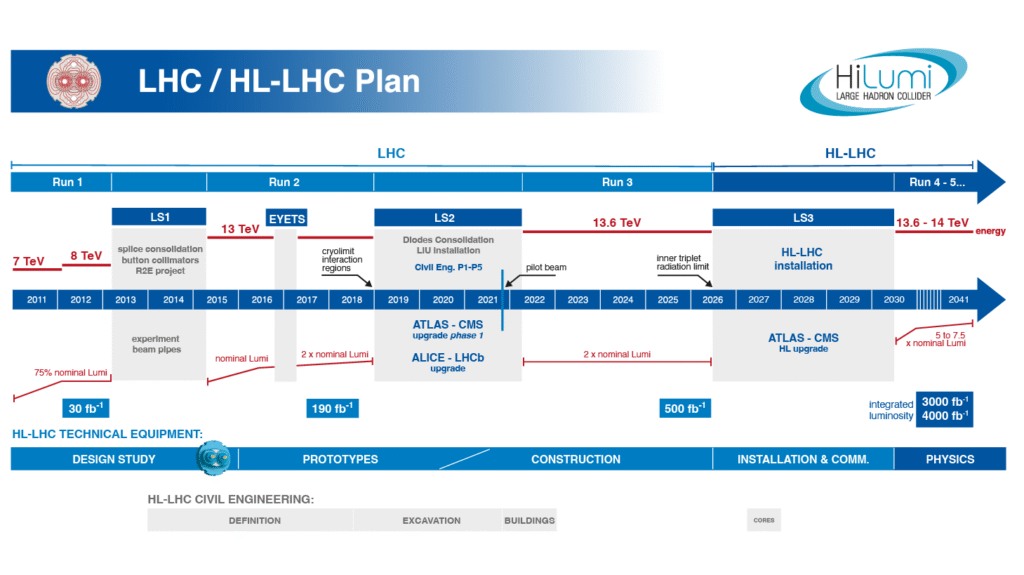
\includegraphics[width=0.8\textwidth]{../images/HL-LHC_calendar.png}
    \caption{Calendario di LHC e HL-LHC. \\ \todo{citare https://hilumilhc.web.cern.ch/about-hilumi-lhc/}}
    \label{fig:hllhc_schedule}
\end{figure}
 
Il calendario è stato rivisto più volte. La presa dati del Run~3 è proseguita fino al 29 giugno 2026~\cite{CERN:AccReport}, mentre il Long Shutdown~3 (LS3) è partito a luglio 2026 e l'avvio di HL-LHC (Run~4) è previsto per giugno 2030~\cite{CERN:LS3}. L'HL-LHC dovrebbe operare dal 2030 al 2041, con presa dati fino all'inizio degli anni 2040~\cite{ESPP:2026}.
 
\subsection{Cosa HL-LHC non potrà fare}
Per quanto HL-LHC rappresenti un salto in avanti nella precisione e nel potenziale di scoperta (fornirà più di cinque volte i dati di LHC, secondo la Strategia 2026~\cite{ESPP:2026}), presenta comunque limiti intrinseci dovuti alla natura adronica del collider:
\begin{itemize}
    \item Le precisioni attese sugli accoppiamenti dell'Higgs sono dell'ordine di pochi per cento, e non si possono eseguire misure dirette o model-independent della larghezza totale del bosone di Higgs (le proiezioni di HL-LHC assumono $|\kappa_V|\le 1$~\cite{FCC:FSR-v1});
    \item l'accoppiamento a quark leggeri come il $c$ resta fuori portata;
    \item i canali rari come $H\to\mu\mu$ o $H\to Z\gamma$ sono misurati con precisioni limitate.
\end{itemize} 
Per rispondere alle domande aperte oltre la portata di HL-LHC sono necessari progressi in precisione e in energia~\cite{ESPP:2026}.
 
\subsection{La Strategia Europea}
Il percorso verso un collider successivo è guidato dalla Strategia Europea per la Fisica delle Particelle. L'aggiornamento 2020 aveva sostenuto il valore scientifico di una Higgs factory $e^+e^-$ seguita da un collider protone-protone alla massima energia raggiungibile, e raccomandato di studiare la fattibilità di FCC come macchina elettrone-positrone come primo stadio (FCC-ee)~\cite{ESPP:2020,ESPP:2026}. Lo studio di fattibilità si è concluso con successo nel 2025~\cite{ESPP:2026}.

Il CERN ha adottato l'aggiornamento del 2026 della Strategia~\cite{ESPP:2026-Res,CERNCourier:ESPP2026}. Il documento conferma che lo sfruttamento completo di LHC e il completamento dell'upgrade HL-LHC sono la massima priorità per gli studi di fisica delle particelle in europa, e che la conclusione di questo programma nei tempi previsti è essenziale per la realizzazione del successivo collider di punta. FCC-ee viene in questo senso raccomandato come opzione preferita per il prossimo collider di punta del CERN~\cite{ESPP:2026}. La decisione sulla costruzione di FCC-ee è prevista per il 2028~\cite{CERNCourier:ESPP2026}.

\section{The Future Circular Collider}
\label{sec:fcc}
La combinazione delle due macchine permette di ottenere una precisione senza precedenti per testare il modello standard e al tempo stesso una forte sensibilità indiretta a nuova fisica. A FCC-ee è prevista la produzione di $\sim3\times10^6$ di bosoni di Higgs, permettendo misure di precisione di massa, larghezze e accoppiamenti a Z, W, $\tau$, b, e c; a FCC-hh è invece prevista la produzione di $\sim20\times10^9$ di bosoni di Higgs, completando il quadro sull'accoppiamento dell'Higgs, del top (Yukawa) e sui modi rari e invisibili. Il programma riassunto ha iniziato a delinearsi dal 2012 ed è culminato nel Conceptual Design Report del 2018. Attualmente la proposta prevede 15 anni di FCC-ee, seguiti da 10 anni di interruzione per sostituire la macchina e da 25 anni di FCC-hh.

La conferma ufficiale del progetto è prevista per il 2028.

\subsection{Il collider}
FCC è una delle principali proposte per i futuri collider di particelle. Si tratta di un'infrastruttura di ricerca in due stadi, da realizzare in un nuovo tunnel sotterraneo lungo $90.7\,\mathrm{Km}$ e posizionato $200\,\mathrm{m}$ di profondità. Il primo stadio (FCC-ee) è un collider $e^+e^-$ alla frontiera di intensità, con energie del centro di massa che variano dal polo della Z fino alla soglia di produzione di $t\bar t$. Il secondo stadio (FCC-hh) è un collider adronico alla frontiera di energia, con energie dell'ordine di $100\,\TeV$~\cite{FCC:FSR-v1,ESPP:2026-Res}. Le due macchine risultano complementari: il primo stadio fornisce misure di precisione assolute e model-independent da usare come normalizzazione per il secondo stadio, che estende di un ordine di grandezza il potere di scoperta diretta~\cite{FCC:FSR-v1}.

Gli studi di fattibilità sono iniziati nel 2012 e hanno portato alla pubblicazione nel 2025 del Feasibility Study Report, articolato in tre volumi e comprendente fisica ed esperimenti, acceleratori e infrastrutture tecniche, ingegneria civile, implementazione e sostenibilità~\cite{FCC:FSR-v1}. \todo{Aggiungi e inserisci anche il volume 2 tra le fonti da citare}. Il documento mostra costi e portata ben definiti, con diversi scenari di finanziamento e un calendario ben definito a partire già da 5/7 anni dopo la fine di HL-LHC. Il progetto offre il programma di fisica di precisione più ampio al mondo, con misure di precisione elettrodeboli, dell'Higgs, del top, del sapore e di QCD, e rendendo FCC-ee l'opzione preferita per il prossimo collider di punta del CERN.

Viene prevista anche un alternativa ridotta di FCC-ee, con meno punti di intersezione (due al posto di quattro) e senza run alla soglia $t-\bar t$. Questa opzione riduce il costo di costruzione del 15\% lasciando però la possibilità di annullare le riduzioni se si rendessero disponibili altre risorse~\cite{ESPP:2026-Res}. La decisione definitiva sulla costruzione di FCC-ee è prevista per il 2028~\cite{CERNCourier:ESPP2026}. 

La lunghezza dell'anello permetterà:
\begin{itemize}
    \item di raggiungere per la prima volte la soglia di produzione di top in collisioni $e^+s^-$ e poter quindi studiare tutte le particelle dello SM;
    \item di ottenere la luminosità più alta mai proposta per un collider circolare (che scala con la circonferenza);
    \item di avere un eccellente controllo dell'energia nel centro di massa sia a energia di Z che alla soglia WW, grazie alla depolarizzazione risonante dei fasci.
\end{itemize}

Sono previsti quattro punti di intersezione, corrispondenti a quattro rivelatori anziché due. In questo modo è stato possibile ottimizzare il layout dell'anello con diversi vantaggi:
\begin{itemize}
    \item Un guadagno fino ad un fattore 1.7 in termini di luminosità (a parità di consumo elettrico), ottenendo in 15 anni gli stessi risultati che avrebbero richiesto 25 anni;
    \item La possibilità di soddisfare un numero maggiore di requisiti sui vari rivelatori che possono quindi controllarsi i risultati a vicenda,
    \item La riduzione delle incertezze sistematiche, che scalano come $1/\sqrt{N_{esperimenti}}$;
    \item La possibilità di monitorare i parametri del fascio grazie all'alto tasso di collisioni alla Z;
    \item La possibilità di accedere a una scoperta a $5\,\sigma$ dell'autoaccoppiamento del bosone di Higgs o dello Yukawa dell'elettrone, che resterebbero poco oltre i $2\,\sigma$ con due soli punti di interazione.
\end{itemize}

\subsection{FCC-ee}
Nella configurazione elettrone-positrone, FCC-ee offre un ambiente pulito rispetto ai collider adronici, muonici e persino lineari, con fasci che si incrociano milioni di volte prima di interagire e l'energia del centro di massa è ben definita e controllabile (effetti di bremmstrahlung e radiazione di sincrotrone contenuti)~\cite{FCC:FSR-v1}. La radiazione di sincrotrone è ulteriormente ridotta grazie all'uso di anelli asimmetrici attorno ciascun punto di interazione, così da evitare l'uso di forti magneti di curvatura a monte. 

La forte focalizzazione lascia uno spazio di appena $2.2\,\mathrm{m}$ e l'insieme di solenoidi e magneti superconduttori si trovano in un cono morto in avanti di $100\,\mathrm{mrad}$ che permette una copertura dino a $\cos\theta\approx0.99$. I solenoidi si spingono fino a $2\,\mathrm{T}$ all'energia di Z, per non aumentare l'emittanza verticale, e fino a $3\,\mathrm{T}$ a energie più elevate.

Le dimensioni trasverse dei fasci permettono un tubo a vuoto di $10\,\mathrm{mm}$ di raggio: la grande vicinanza del primo strato di del rivelatore permette di ottimizzare il tagging di b e c. Il pile-up è inoltre ridotto a circa $2\times10^{-3}$ alla Z e a meno di $10^{-2}$ alle energie del top.

Le condizioni di lavoro di FCC definiscono alcuni requisiti che i futuri rivelatori devono soddisfare. Il tasso di eventi previsto supera i $100\,\mathrm{kHz}$ al polo della Z; lo studio delle coppie WW e del sapore richiede un'ottima risoluzione della calorimetria elettromagnetica. Sono attualmente in studio tre concept principali (CLD, IDEA, ALLEGRO).

\subsubsection{Regimi di lavoro}
Il programma prevede quattro punti di lavoro da esplorare in circa quindici anni di funzionamento: polo della Z, soglia WW, massimo di sezione d'urto di produzione ZH e regione del top. Vengono riportati in tabella~\ref{tab:soglie} i valori sommati sui quattro rivelatori, tenendo conto di 185 giorni di fisica all'anno con efficienza operativa del $75\%$~\cite{FCC:FSR-v1}.

\begin{table}[hbtp]
    \centering
    \resizebox{\textwidth}{!}{
    \begin{tabular}{lcccc}
        \hline
        & Polo della Z & Soglia WW & ZH & $t\bar t$ \\
        \hline
        $\sqrt{s} \,(\GeV)$ & 88, 91, 94 & 157, 163 & 240 & 340–350, 365 \\
        $\mathcal{L} \,(\frac{10^{34}}{\mathrm{cm^2\,s}})$ & 140 & 20 & 7.5 & 1.8, 1.4 \\
        Durata (anni) & 4 & 2 & 3 & 1, 4 \\
        $\mathcal{L}_{\text{integrata}} \,(\mathrm{ab^{-1}})$ & 205 & 19.2 & 10.8 & 0.42, 2.70 \\
        Eventi attesi & $6\times10^{12}$ & $2.4\times10^{8}$ & $2.2\times10^{6}$ {\small di ZH} & $2\times10^{6}$ {\small di $t\bar t$} \\
        & & & 65k {\small di WW} $\rightarrow$ {\small H} & 370k {\small di ZH} \\
        & & & & 92k {\small di WW} $\rightarrow$ {\small H} \\
        \hline
    \end{tabular}
    }
    \caption{Parametri operativi e prestazioni previste per i diversi punti di lavoro del FCC.}
    \label{tab:soglie} 
\end{table}

In totale si prevede di produrre $6\times10^{12} Z, 2.4\times10^{8}$ coppie W, quasi $3\times10^{6}$ bosoni di Higgs e $2\times10^{6}$ coppie di top~\cite{FCC:FSR-v1}. Questo è l'insieme più ristretto di energie che permettano di studiare tutte le particelle dello SM.

\paragraph{Polo della Z:} permette di accedere alla fisica del sapore, di QCD e di adronizzazione (b, c $\tau$) grazie alla produzione massiva di bosoni Z ($5\times10^{12}$ in un paio di anni), che permetteranno anche la ricerca di eventi rari o proibiti. I run a 88 e 94~$\GeV$ permetteranno di raccogliere intorno ai $40\,ab^{-1}$ di dati, accedendo a misure di precisione della Z e di altre osservabili elettrodeboli migliorando la risoluzione attuale di un fattore 50-1000. Aumentando la precisione su misure come $\alpha_{QED}(m_Z)$ e $\alpha_S(m_Z)$ si possono superare le limitazioni nell'interpretazione di misure successive come quelle di $sin^2\theta_W$.
\paragraph{Soglia WW:} permette misure di precisione di massa e larghezza del W accumulando almeno $20\,ab^{-1}$ di dati in un paio di anni. Tramite questi si può accedere al numero di specie di neutrini e ad una misura indipendente di $\alpha_S$.
\paragraph{Energia di produzione di ZH:} permette di raccogliere $10\,ab^{-1}$ di dati in tre anni lavorando all'energia ottimizzata per l'Higgsstrahlung ($240\,\GeV$). Questi permettono di misurare in modo model-independent gli accoppiamenti del bosone di Higgs (in particolare l'accoppiamento alla Z).
\paragraph{Soglia $t-\bar t$:} permette di accedere a misure di massa del top, con una precisione dell'ordine di $10\,\MeV$. Massa top è attualmente una delle maggiori limitazioni nello sudio delle osservabili elettrodeboli. Per raggiungere la massima sensibilità e aumentare la portata sulla scala di nuova fisica (potenzialmente fino a un 60\%) serve eguagliare l'incertezza statistica su massa W ($180\,\keV$) e massa Z ($4\,\keV$), rispettivamente con 20 e 15~$\MeV$ su $m_{top}$.
\paragraph{Soglia a $365\,\GeV$:} permette di dare sensibilità all'autoaccoppiamento dell'Higgs, aprendo la possibilità a scoperta a $5\,\sigma$. Con queste misure è possibile anche eguagliare la precisione al polo della Z anche sugli accoppiamenti elettrodeboli del top, mantenendo l'incertezza teorica sullo Yukawa del top al per cento anche a FCC-hh.

La "Quasi-totalflexibility" permette di scegliere un ordine di run diverso da quello presentato con energie successive~\cite{FCC:FSR-v1}. Nel periodo fino alla fine del 2027 sono inoltre previsti studi per aumentare le luminosità a tutte le energie~\cite{FCC:FSR-v1}.

\subsubsection{Programma di fisica}
Il programma di fisica punta a diversi obiettivi, legati alle domande fondamentali della fisica:
\begin{itemize}
    \item Verificare con la massima precisione che tutte le misure dell'Higgs siano compatibili con la versione dello SM della EWSB, e affrontare il problema della naturallezza della massa dell'Higgs con misure al per mille degli accoppiamenti;
    \item misurare l'autoaccoppiamento dell'Higgs (l'asimmetria materia-antimateria potrebbe dipendere da una modifica del potenziale di Higgs che fornisce una transizione di fase elettrodebole (EW) del primo ordine) e, con alta luminosità, cercare direttamente leptoni neutri pesanti;
    \item misurare accoppiamenti di seconda e terza famiglia con precisione inferiore al per cento (per cercare spiegazioni allo schema degli accoppiamenti di Yukawa) e effettuare prime misure di strange e di sensibilità allo Yukawa dell'elettrone;
    \item migliorare di uno o più ordini di grandezza la sensibilità ai coefficienti EFT per cercare nuova fisica BSM. 
\end{itemize}

\subsubsection{Fisica dell'Higgs}
La produzione del bosone di Higgs è massimizzato all'energia di $240\,\GeV$ dove domina il processo di Higgsstrahlung, $e^+e^-\rightarrow ZH$, insieme con la WW-fusion. A questi regimi è prevista la produzione di $approx\,3\times10^6$ bosoni di Higgs, che permetteranno di misurare in modo model-independent diversi accoppiamenti con precisione del per mille, la larghezza totale con precisioni inferiori al per cento e la massa con precisione di pochi $\MeV$~\cite{FCC:ESPPU-physics}. È possibile misurare la sezione d'urto $\sigma_{ZH}$ contando gli eventi in cui la massa di recoil $m^2_{recoil}\,=\,2\,+\,m^2_Z\,-\,2\sqrt{sE_Z}$ identifica una Z, indipendentemente dal decadimento dell'H. Questa misura fornisce il valore di $k_Z$, fondamentale come riferimento per le misure successive e, dalla posizione del picco, il valore di massa del bosone di Higgs. Vale inoltre $\alpha_{ZH}\times BR_{H\rightarrow ZZ}\propto\frac{k^4_Z}{\Gamma_H}$, quindi dalla misura di $\sigma_{ZH}$ si può accedere anche alla larghezza totale in modo model-independent~\cite{FCC:FSR-v1,FCC:ESPPU-physics}. 

Le proiezioni prevedono una precisione di $0.31\%$ su $\sigma_{ZH}$ a $240\,\GeV$, $0.52\%$ a $254\,\GeV$ e di circa $4\,\MeV$ (dominata dalla statistica, $2\,\MeV$ di sistematica) su $m_H$ come mostrato in Tabella \ref{tab:precisioni}.

\begin{table}
    \centering
    \begin{tabular}{cccc}
        \hline
        Parametro & HL-LHC\tablefootnote{assumendo $|k_V|\leq1$} & FCC-ee & FCC-ee + FCC-hh \\
        \hline
        $k_Z$ (\%)       & 1.3 & 0.10 & 0.10 \\
        $k_W$ (\%)       & 1.5 & 0.29 & 0.25 \\
        $k_b$ (\%)       & 2.5 & 0.38 & 0.33 \\
        $k_\tau$ (\%)    & 1.6 & 0.46 & 0.40 \\
        $k_c$ (\%)       &     & 0.70 & 0.68 \\
        $k_\gamma$ (\%)  & 1.6 & 1.1  & 0.30 \\
        $k_Z\gamma$ (\%) & 10  & 4.3  & 0.67 \\
        $k_t$ (\%)       & 3.2 & 3.1  & 0.75 \\
        $k_\mu$ (\%)     & 4.4 & 3.3  & 0.42 \\
        $k_H$ (\%)       &     & 0.78 & 0.69 \\
        \hline
    \end{tabular}
    \caption{Precisioni attese per HL-LHC, FCC-ee e per l'intero programma di FCC. Precisione relativa al 68\% CL, con 4 punti di interazione e alla luminosità di riferimento~\cite{FCC:FSR-v1}}
    \label{tab:precisioni}
\end{table}

Il programma di precisione dell'Higgs si completa in tre anni di run a $240\,\GeV$, o in otto comprendendo anche la run a $365\,\GeV$~\cite{FCC:FSR-v1}.

La precisione del per cento richiesta è necessaria per cercare nuova fisica BSM la cui scala corrisponde a $E_{max}\,\approx\,\frac{1.1\,\TeV}{\sqrt{k_Z-1}}\,\approx\,15\,\TeV$, che è alla portata di FCC-hh: una deviazione dello $0.5\%$ a HL-LHC corrisponde a $0.5\,\sigma$, ma a FCC-ee corrisponderebbe a $5\,\sigma$, quindi a una scoperta. 

A FCC-ee i contributi radiativi a un loop di $k_\lambda$ alle sezioni d'urto dell'Higgs possono essere misurate con precisione del per cento a $240\,\GeV$ e $365\,\GeV$, che combinata con le misure di HL-LHC porta a una precisione del $15\%$ ($18\%$ senza raddoppiare la luminosità, $28\%$ in autonomo). 

Insieme allo Yukawa dell'elettrone, la produzione risonante $e^+e^-\rightarrow H$ a $\sqrt{s}\,=\,125\,\GeV$ darebbe accesso anche a H-invisibile, violazione di CP nell'accoppiamento HZZ e i decadimenti $H\rightarrow\gamma\gamma, H\rightarrow\gamma Z, H\rightarrow\mu\mu$ insieme con $\gamma H$.

Le misure di diboson vincolano gli anomalous triple gauge coupling, che sono a loro volta correlati agli accoppiamenti dell'Higgs ai bosoni vettori, con precisione assoluta di $10^{-3}$~\cite{FCC:ESPPU-physics}. Le misure al polo della Z solo complementari a quelle di energia più alta: l'enorme precisione ottenuta a $90\,\GeV$ vincola operatori che entrano solo a loop ed in modo diverso dalle misure sopra il polo.

\subsubsection{Fisica di precisione nel settore EW}
Un miglioramento di un fattore 50 nella precisione della lineshape di Z si traduce in un miglioramento di un fattore 7 in scala di energia. L'effetto di particelle pesanti debolmente accoppiare di rivela fino a masse di diverse decine di $\TeV$. In Tabella \ref{tab:osservabili} viene riportata una selezione di osservabili.

\begin{table}
    \centering
    \begin{tabular}{cccc}
        \hline
        Osservabile & Valore attuale & Incertezza stat & Incertezza sis \\
        \hline
        $m_Z$ [$\keV$]                 & 91 187 600 $\pm$ 2000 & 4    & 100  \\
        $\Gamma_Z$ [$\keV$]            & 2 495 500 $\pm$ 2300  & 4    & 12   \\
        $\sin^2_{\Theta^{eff}}$ ($\times10^6$) & 231 480 $\pm$ 160     & 1.2  & 1.2  \\
        $1/\alpha_{QED}(m_Z^2)$ ($\times10^3$) & 128 952 $\pm$ 14      & 3.9  & {\small \todo{piccola}} \\
        $R_{\textit{l}^Z}$ ($\times10^3$)      & 20 767 $\pm$ 25       & 0.05 & 0.05 \\
        $\alpha_{S}(m_Z^2)$ ($\times10^4$)     & 1196 $\pm$ 30         & 0.1  & 1    \\
        $N_\nu$ ($\times10^3$)                 & 2996.3 $\pm$ 7.4      & 0.09 & 0.12 \\
        $m_W$ [$\MeV$]                 & 80 360.2 $\pm$ 9.9    & 0.18 & 0.16 \\
        $\Gamma_W$ [$\MeV$]            & 2085 $\pm$ 42         & 0.27 & 0.2  \\
        $m_t$ [$\MeV$]                 & 172 570 $\pm$ 290     & 4.2  & 4.9  \\
        $\Gamma_t$ [$\MeV$]            & 1420 $\pm$ 190        & 10   & 6    \\
        \hline
    \end{tabular}
    \caption{Diverse osservabili misurate a FCC-ee}
    \label{tab:osservabili}
\end{table}

Le misure dirette di $\alpha_{QED}(m_Z^2)$ e $\alpha_{S}(m_Z^2)$ sono importanti, perché altrimenti dominerebbero le incertezze parametriche di tutti i calcoli di precisione del SM. Le principali sistematiche sono la calibrazione dell'energia dei fasci e la luminosità; in generale ci si aspetta di portare le incertezza sistematiche al livello delle statistiche~\cite{FCC:FSR-v1}.

Massa e larghezza del W sono ottenute dal profilo della sezione d'urto vicino alla soglia e dalla ricostruzione cinematica; le misure delle frazioni di decadimento leptoniche del W arrivano a una precisione di $1.3\times10^{-4}$~\cite{FCC:ESPPU-physics}. Dalla produzione di coppie W si può misurare anche l'accoppiamento della Z al neutrino elettronico con un incertezza statistica di $0.7\%$.

\subsubsection{Fisica del top}
Alla soglia $t-\bar t$ è possibile misurare massa e larghezza del top con incertezze dell'ordine di $10\,\MeV$~\cite{FCC:FSR-v1} ($6.5\,\MeV$ su $m_{top}$ e $11.5\,\MeV$ su $\Gamma_{top}$), con limite dato dall'incertezza teorica e dall'accoppiamento di Yukawa del top assunto noto al $3\%$ da HL-LHC. Alla soglia a $365\,\GeV$ si possono misurare gli accoppiamenti elettrodeboli ttZ con precisione di $0.5-1.5\%$ e vincolare lo Yukawa del top al $2.1\%$; queste misure servono per normalizzare ttH a ttZ a FCC-hh, così da ottenere lo Yukawa del top al per cento~\cite{FCC:FSR-v1}.

\subsubsection{Fisica del sapore, QCD e delle particelle debolmente accoppiate}
La fisica del sapore è resa possibile dall'enorme campione di Z e dal raggio minore del tubo a vuoto; grazie a questi aspetti è possibile migliorare di un fattore 2000 le osservabili di sapore come $R_b, R_c, A_{FB}^b e A_{FB}^c$. È inoltre possibile misurare la costante di Fermi con precisione del $10^{-5}$ a partire da massa, vita media e rapporti di decadimento del $\tau$.

FCC-ee inoltre estende la regione di scoperta di eventuali leptoni neutri pesanti fino alle regioni fisicamente favorite dai modelli seesaw, e quella di ricerca di mono-fotoni e missing energy per modelli come WIPM leptofilici o ricercare particelle a lunga vita e decadimenti esotici di Higgs e Z. Infine permette di esplorare quasi interamente l'accoppiamento HZZ, che potrebbe nascondere transizioni di fasi elettrodeboli del primo ordine.

\subsubsection{Luminosità}
La luminosità ($\mathcal{L}$) è una grandezza fondamentale che descrive le prestazioni di un collisore o di un fascio di particelle. Quantifica la probabilità che avvengano interazioni (collisioni) tra le particelle dei fasci incidenti, disaccoppiando le caratteristiche geometriche e cinematiche della macchina acceleratrice dalla fisica microscopica del singolo processo d'urto. La luminosità instantanea $\mathcal{L}$ (in $\mathrm{cm}^{-2}\mathrm{s}^{-1}$) collega la sezione d'urto $\sigma$ di un processo al numero di eventi prodotti per unità di tempo secondo $\frac{dN}{dt}\,=\,\sigma\mathcal{L}$, misurando il flusso di particelle incidenti per unità di area e di tempo. Integrando nel tempo si ottiene $N\,=\,\sigma\mathcal{L}_{int}$, dove con $\mathcal{L}_{int}$ ci si riferisce alla luminosità integrata, esperessa in $ab^{-1}$. In base al valore di luminosità cambiano le misure accessibili e la rispettiva incertezza (l'incertezza statistica scala come $1/\sqrt{N}$, ma va anche considerato che molte misure hanno incertezze sistematiche che migliorano con i dati (campioni di controllo e calibrazioni)).

A FCC-ee sono previste luminosità nell'ordine degli $\mathrm{ab}$, come mostrato in Tabella \ref{tab:luminosità}.

\begin{table}
    \centering
    \begin{tabular}{c|cccc}
         & Z & WW & ZH & $t\bar t$ \\
        \hline
        $E_{beam}$ [$\GeV$]                            & 45.6  & 80   & 120  & 182.5 \\
        $\mathcal{L}$ [$10^{30} \mathrm{cm}^{-2}s^{-1}$]       & 145   & 20   & 7.5  & 1.41  \\
        Corrente [$\mathrm{mA}$]                               & 1294  & 135  & 26.8 & 5.1   \\
        Numero pacchetti                                       & 11200 & 1852 & 300  & 64    \\
        Distanza pacchetti [$\mathrm{ns}$]                     & 27    & 163  & 1008 & 4725  \\
        $\sigma_x$\tablefootnote{al punto di intersezione} [$\mathrm{\mu m}$] & 9.5   & 21.8 & 12.6 & 36.9  \\
        $\sigma_x$\footnotemark[\value{footnote}] [$\mathrm{nm}$]    & 40.1  & 44.7 & 31.6 & 43.6  \\
        Dispersione E ($\sigma_\delta$) [\%] & 0.039/0.121 & 0.069/0.105 & 0.102/0.176 & 0.151/0.184 \\ 
    \end{tabular}
    \caption{Parametri chiave del collider ai quattro punti di lavoro, consideando quattro punti di intersezione}
    \label{tab:luminosità}
\end{table}

Vengono predisposti appositi accorginemti per raggiungere questi risultati:
\begin{itemize}
    \item la luminosità è direttamente proporzionale alla circonferenza dell'anello, e a questo si aggiunge che i fasci si incrociano molte volte prima di interagire;
    \item la luminosità decresce come il quadrato dell'energia a causa della radiazione di sincrotrone ($\mathcal{L}\propto\frac{P_{SR}}{E^2}$), causando un crollo della luminosità di due ordini di grandezza nel passaggio dalla soglia della Z a quella del top (la potenza è mantenuta costante riducendo il numero di pacchetti);
    \item si sfrutta la tecnica del "crab-waist" e si sfruttano angoli molto grandi ($30\,\mathrm{mrad}$) al punto di intersezione;
    \item un acceleratore di iniezione rifornisce costantemente i fasci permettendo di tenere la luminosità al picco, compensando la bassa vita dei fasci (pochi minuti, a causa di processi radiativi). FCCee continuerebbe a raccogliere dati anche durante l'iniezione~\cite{FCC:FSR-v1}.
\end{itemize}

Il passaggio da $\mathcal{L}$ a $\mathcal{L_{int}}$ richiede un modello di funzionamento: vengono assunti 185 giorni di fisica all'anno e un efficienza operativa del $75\%$ ($1.2\times10^7$ secondi di collisioni all'anno)~\cite{FCC:FSR-v1}.

\begin{table}
    \centering
    \begin{tabular}{c|cccc}
         & Z & WW & ZH & $t\bar t$ \\
        \hline
        $\mathcal{L}_{annua}$ [$ab^{-1}$]     & 68  & 9.6  & 3.6  & 0.83/0.67 \\
        Durata [years]                        & 4   & 2    & 3    & 1/4       \\
        $\mathcal{L}_{int}$\footnotemark\ [$ab^{-1}$] & 205 & 19.2 & 10.8 & 0.42/2.70 \\
    \end{tabular}
    \label{tab:valLumi}
    \caption{Luminosità integrata annua e totale, sommata sui quattro punti di interazione}
\end{table}

\footnotetext{Durante la fase iniziale di ogni blocco la luminosità è ridotta: i primi due anni alla Z e in primo a $t\bar t$ sono assunti a luminosità dimezzata. Per questo il totale non corrisponde alla prodotto $\mathcal{L}_{annua}\times$Durata; inoltre sono considerati periodi di fermo per preparare la run ai run successivi.}

A partire dalla luminosità si può ottenere il numero di eventi attesi per un processo come $N\,=\,\sigma\mathcal{L}_{int}\epsilon$, con $\epsilon$ efficienza. In tabella \ref{tab:evProdotti} sono riportati i numeri di eventi prodotti in tutto il programma.

\begin{table}
    \centering
    \begin{tabular}{c|cc}
        Punto di lavoro & $\mathcal{L}_{int}$ [$ab^{-1}$] & $N_{ev}$                           \\
        Z               & 205                             & $6\times10^{12}$ Z                 \\
        WW              & 19.2                            & $2.4\times10^{12}$ WW              \\
        ZH              & 10.8                            & $2.2\times10^{12}$ ZH              \\
                        &                                 & $6.5\times10^{4}$ WW$\rightarrow$H \\
        $t\bar t$       & 0.42+2.70                       & $2\times10^{12}$ $t\bar t$         \\
                        &                                 & $3.7\times10^{5}$ ZH               \\
                        &                                 & $9.2\times10^{4}$ WW$\rightarrow$H \\

    \end{tabular}
    \caption{Eventi previsti ad ogni punto di lavoro, considerando 4 punti di intersezione.}
    \label{tab:evProdotti}
\end{table}

Queste grandi statistiche di traducono in precisioni considerevoli, come viene dichiarato nel Feasibility Study e nel contributo ESPPU25. Gli errori statistici sono nell'ordine di $10^{-6}$ sulla lineshape della Z e a $1.5\times10{12}$ per punto di intersezione; $0.31\%$ su $\sigma_{ZH}$ a $240\,\GeV$ e circa $4\,\MeV$ su $m_H$; $0.18\,\MeV$ (stat) su $m_W$. 

Grazie all'aumento di luminosità è poossibile portare oltre i $2\,\sigma$ (e fino ai $5\,\sigma$ richiesti per la scoperta) l'autoaccoppiamento dell'Higgs, la misura dello Yukawa dell'elettrone e la ricerca completa dei neutrini sterili; è inoltre possibile parlare di scoperta in soli 4 anni anche alla produzione risonante $e^+e^-\rightarrow H$, dove si richiede di ridurre la luminosità per ridurre la dispersione di energia dei fasci, con una significatività di $2.6\,\sigma$ l'anno. L'alta luminosità permette di raccogliere in un giorno di lavoro i $10^9$ Z necessari per mitigare l'incertezza elettrodebole sull'Higgs, e di arrivare nei tempi previsti ai $10^{12}$ richiesti per la fisica del sapore e per lo studio delle osservabili EW. Con un ulteriore aumento della luminosità integrata a $240\,\GeV$ e $340\,\GeV$ (facendo run più lunghe) si potrebbe portare l'incertezza su $k_\lambda$ dal $18\%$ al $15\%$

\paragraph{La misura della luminosità} è effettuata tramite due processi distinti: scattering Bhabha a piccolo angolo ($e^+e^-\rightarrow e^+e^-$) e produzione di coppie di fotoni a grande angolo ($e^+e^-\rightarrow\gamma\gamma$), che ci si aspetta essere rilevanti per FCC-ee. Ci si aspetta di poter misurare $\mathcal{L}$ con precisioni nell'ordine del $10^{-4}$ sulla luminosità assoluta, e del $10^{-5}$ sulla luminosità integrata.

La combinazione di precisione e luminosità permette infine di ottenere sensibilità indiretta a nuova fisica dino a una scala di $100\,\TeV$ (considerando descrizione EFT con operatori di dimensione 6) o anche di più (considerando modelli diversi \todo{famo un check, dai}). Già il run alla Z ha buone possibilià di individuare tracce in eventuali modifiche delle osservabili con potenziale di scoperta per quasi ogni scenario che porti a modifiche nel SM a tree-level, anche con particelle di diverse decine di TeV, vincolando già operatori che entrano solo a loop. 

\subsection{FCC-hh}
Il secondo stadio, FCC-hh, è un collider adronico che lavorerà a energie comprese tra gli ottanta e i cento $\TeV$, estendendo la misura delle proprità dell'Higgs a processi che presentano accoppiamenti efficaci più piccoli (decadimenti rari come $\gamma\gamma$, $\mu\mu$ o $Z\gamma$) o che richiedono energie maggiori ($t\bar tH$ e $HH$) e esplorando direttamente scale multi-TeV ben superiori alla scala della SSB, per studiare eventuali deviazioni trovate a FCC-ee e allargare la portata di massa per un ampia classe di teorie BSM. Grazie alla produzione di oltre $2\times10^{10}$ bosoni di Higgs, gli accoppiamenti piccoli sono determinati in valore assoluto con precisione inferiore al per cento (sfruttando i rapporti con gli accoppiamenti già misurati nello stadio FCC-ee), mentre l'autoaccoppiamento sarà misurato con precisione inferiore al $5\%$. 

Per quanto riguarda la scoperta diretta, è previsto che la portata arrivi a $40\,\TeV$ per risonanze in canale s, $10-20\,\TeV$ per particelle fortemente interagenti. Prevede inoltre misure di precisione a grande $Q^2$ come misure di sezione d'urto differenziali di $t\bar t$ (incertezza inferiore al $10\%$ fino a $m_{inv}\approx30\,\TeV$), di WW (fino a $8.5\,\TeV$) e di tttt (al $4\%$). 

A FCC-hh sarà possibile operare anche collisioni piombo-piombo fino a $40\,\TeV$ per studiare il plasma QCD ad alta densità e temperatura~\cite{FCC:FSR-v1}.

Per tutte le misure di FCC-hh rimane comunque indispensabile la sinergia con FCC-ee per sfruttare al massimo le misure di rapporti raccolte da FCC-hh. Inoltre alcuni tipi di nuova fisica sono visibili sono a uno dei due.


\begin{comment}
**Incongruenze da risolvere**
- **κ_W di FCC-ee**: il testo del Feasibility Study (§1.1) dice 0.23%, la sua tabella 3 e la sezione 2.5 dicono 0.29%. Ho usato la tabella.
- **Energia di FCC-hh**: il CDR usa 100 TeV, il Feasibility Study studia 80-120 TeV, il contributo ESPPU25 usa 84 TeV. Scelgo 100 come baseline.
- **Durata dei run al top**: il Feasibility Study dà 1 anno a 340-350 GeV e 4 anni a 365 GeV (totale 5 anni, 3.12 ab⁻¹ come somma); ESPPU25 le accorpa in 5 anni.
- **Luminosità per punto di interazione**: due tabelle del Feasibility Study danno valori lievemente diversi (140 oppure 145×10³⁴ alla Z; 1.4 oppure 1.41 al top); altri documenti riportano valori leggermente diversi, perché sono parametri preliminari (per esempio 182 o 181×10³⁴ alla Z).
- **Durata del programma**: il Feasibility Study parla di 15 anni di FCC-ee, mentre alcuni documenti per la Strategia contano 14 anni di funzionamento più circa un anno e mezzo di messa in servizio.

**Lacune e cose da verificare**
- Per i dettagli di acceleratore (sistema RF, criogenia, potenza, magneti) servirebbe il vol. 2 del Feasibility Study, che non ho consultato. Per tunnel e ingegneria civile il vol. 3.
- I numeri su tunnel, profondità, siti, costi e calendario vengono da pagine CERN: citali dal vol. 3 o dal comunicato CERN originale.
- Lascio fuori i confronti con altri collider, le tre sezioni del Feasibility Study sulla fisica del sapore nel dettaglio e sul forward-physics facility.
- Il confronto "mezzo secolo contro 3-8 anni" con altri Higgs factory è un confronto con altri progetti.
\end{comment}


\begin{comment}
# Modello Standard e Vector Boson Scattering: materiale di base per la tesi
**Sigle delle fonti**
- **[Cov21]**: R. Covarelli, M. Pellen, M. Zaro, *Vector-Boson Scattering at the LHC: unravelling the Electroweak sector*, Int. J. Mod. Phys. A 36 (2021) 2130009, arXiv:2102.10991. È una rassegna di riferimento sul VBS (e uno degli autori è dell'Università di Milano).
- **[Apy22]**: slide di A. Apyan, *VBS and VVV studies at future colliders* (Energy Frontier Workshop, Snowmass, 2022). Sono slide: dove possibile cita i lavori originali.
- **[Fle17]**: C. Fleper, W. Kilian, J. Reuter, M. Sekulla, *Scattering of W and Z bosons at high-energy lepton colliders*, Eur. Phys. J. C (2017), DOI 10.1140/epjc/s10052-017-4656-5, arXiv:1607.03030.
- **[FSR §x]**, **[ESPPU25]**, **[ESPP26]**: come nel file su FCC.
- **[standard]**: risultato di testo (Peskin-Schroeder, Schwartz, Langacker, PDG) che non ho preso da una fonte specifica tra quelle lette. Va citato da un libro o dalla rassegna del PDG, e conviene controllare le formule.
\end{comment}

\section{The Standard Model}
Il Modello Standard (SM) è una teoria quantistica di campo basata sui principi di invarianza di Lorentz, località e simmetrie di gauge, ed è in grado di spiegare un intervallo enorme di fenomeni, dalla spettroscopia atomica alle collisioni ad alte energie.

In questa descrizione, le forze sono rappresentate da campi di gauge con gruppo di simmetria $SU(3)_C\otimes SU(2)_L\otimes U(1)_Y$ (associati, rispettivamente, a colore, isospin debole e ipercarica). Per il settore elettrodebole si ha $SU(2)_L\otimes U(1)_Y$. La materia è invece definita da campi di spin 1/2, ossia i quark (tripletti di colore) e leptoni (singoletti di colore), entrambi divisi in 3 famiglie con stessi numeri quantici ma masse diverse. In ogni famiglia i campi sono organizzati in doppietti che differiscono per carica elettrica.

Le interazioni di gauge del SM sono chirali: solo i doppietti sinistrorsi sono carichi sotto $SU(2)_L$, quindi le interazioni con i campi $SU(2)_L\otimes U(1)_Y$ dipendono dall'elicità dei fermioni. Nel SM non sono massless e sinistrorsi, per neutrini massivi e destrorsi serve fisica BSM.

La scoperta nel 2012 del bosone di Higgs da parte di ATLAS e CMS ha completato il quadro dello SM, che risulta oggi una teoria completa e consistente. Nonostante questo rimangono però fenomeni che non sono spiegati dallo SM, come la dominanza della materia sull'animateria, il pattern delle masse dei fermioni e le oscillazioni dei neutrini. \todo{Inseriamo qua la famosa immagine dello SM}

\paragraph{Settore elettrodebole} Il settore elettrodebole è descritto da $$\mathcal{L}_{\mathrm{EW}} = -\tfrac14 W^a_{\mu\nu}W^{a\,\mu\nu} - \tfrac14 B_{\mu\nu}B^{\mu\nu} + \sum_\psi \bar\psi\, i\slash{D}\,\psi + (D_\mu\Phi)^\dagger (D^\mu\Phi) - V(\Phi) + \mathcal{L}_{\mathrm{Yuk}},$$ con derivata covariante $D_\mu = \partial_\mu - i g\, T^a W^a_\mu - i g' Y B_\mu$\footnote{Il segno dipende dalla convenzione}.

Il tensore di campo non abeliano $$W^a_{\mu\nu} = \partial_\mu W^a_\nu - \partial_\nu W^a_\mu + g\,\epsilon^{abc} W^b_\mu W^c_\nu$$ contiene termini cubici e quartici nei campi $W$, che corrispondono agli accoppiamenti doppi e tripli dei bosoni di gauge (autointerazioni). Il campo abeliano $B$ invece non si autoaccoppia.

\paragraph{Problema della massa} Aggiungere un termine di massa per i bosoni di gauge e per i fermioni romperebbe esplicitamente l'inverianza di gauge. Per spiegare l'origine delle masse non si possono usare i soli campi di gauge e fermionici, ma bisogna passare per il meccanismo di rottura spontanea della simmetria elettrodebole (EWSSB). Si può dimostrare che aggiungendo un campo scalare è possibile innescare la EWSSB dando massa ai campi di gauge senza rompere la simmetria a livello della Lagrangiana. Dopo la rottura i campi di isospin e ipercarica si mescolano e danno i mediatori delle interazioni (fotone massless ($\gamma$) e bosoni deboli massivi ($Z$, $W^\pm$)) mentre le interazioni di Yukawa tra campi scalari e fermionici forniscono masse ai fermioni. Quel che rimane del campo scalare è un campo scalare massivo che rappresenta una nuova particella (bosone di Higgs).
\todo{vedi se citare Elitzur nelle footnote}


\begin{comment}
## A.3 La rottura spontanea della simmetria elettrodebole (EWSB)
**Formule essenziali** [standard]:

- Potenziale $V(\Phi) = -\mu^2\,\Phi^\dagger\Phi + \lambda\,(\Phi^\dagger\Phi)^2$, con minimo a $\langle\Phi\rangle = (0,\; v/\sqrt2)^T$.
- Il valore di aspettazione nel vuoto è legato alla costante di Fermi: $v = (\sqrt2\, G_F)^{-1/2} \simeq 246\ \mathrm{GeV}$.
- Dei quattro gradi di libertà di $\Phi$, tre sono bosoni di Goldstone, "mangiati" dai bosoni $W^\pm$ e $Z$ come polarizzazione longitudinale; il quarto è il campo di Higgs $h$.
- Massa dell'Higgs: $m_H^2 = 2\lambda v^2$. Con $m_H = 125.20 \pm 0.11\ \mathrm{GeV}$ (valore usato in [FSR §2.1]) si ricava $\lambda \approx 0.13$ (calcolo mio).
- Masse dei bosoni: $m_W = \tfrac12 g v$, $m_Z = \tfrac12 v\sqrt{g^2+g'^2} = m_W/\cos\theta_W$, con $\tan\theta_W = g'/g$; il fotone resta senza massa e $e = g\sin\theta_W$.
- Masse dei fermioni: $m_f = y_f\, v/\sqrt2$, con $y_f$ costanti di Yukawa libere.
- Accoppiamenti dell'Higgs: ai fermioni proporzionali a $m_f/v$; ai bosoni vettori $g_{HVV} = 2\, m_V^2/v$ e quartico $g_{HHVV} = 2\, m_V^2/v^2$ (in alcune convenzioni, il fattore cambia).
\end{comment}


Una volta nota la massa dell'Higgs, lo SM è in grado di prevedere tutta la fenomenologia dell'Higgs senza ulteriori parametri liberi. La massa misurata è compatibile con questo meccanismo, ma va verificata con ulteriori misure alla massima precisione possibile. Questo meccanismo non è in grado di spiegare lo schema osservato degli accoppiamenti di Yukawa.

\todo{Vediamo se mettere un paragrafo con correnti cariche/neutre e accoppiamenti}

\begin{comment}
## A.4 Correnti e accoppiamenti [standard]

- **Corrente carica**: $\frac{g}{\sqrt2}\, W^+_\mu\, \bar u_L \gamma^\mu V_{\mathrm{CKM}}\, d_L$ + h.c., e l'analoga per i leptoni. Solo componenti sinistrorse.
- **Corrente neutra**: $\frac{g}{\cos\theta_W}\, Z_\mu\, \bar f \gamma^\mu \left(T_3 P_L - Q\sin^2\theta_W\right) f$, con accoppiamenti vettoriali e assiali diversi per ogni fermione; il fotone si accoppia come $e\,Q\,A_\mu$.
- **Autoaccoppiamenti dei bosoni di gauge**: esistono i vertici tripli $WW\gamma$ e $WWZ$ e i quartici $WWWW$, $WWZZ$, $WWZ\gamma$, $WW\gamma\gamma$. **Non** esistono vertici $ZZZ$, $ZZ\gamma$ e $ZZZZ$ a livello albero, perché la struttura non abeliana coinvolge solo la componente $W^3$ insieme a $W^\pm$. È rilevante per il VBS con $ZZ$ nello stato finale: lo scattering $ZZ \to ZZ$ passa a livello albero solo attraverso lo scambio dell'Higgs.
- **Accoppiamenti dell'Higgs ai bosoni vettori**: $HWW$, $HZZ$ e i quartici $HHWW$, $HHZZ$.

**Relazioni a livello albero** [standard]:
- $\dfrac{G_F}{\sqrt2} = \dfrac{g^2}{8\, m_W^2}$;
- $\rho \equiv \dfrac{m_W^2}{m_Z^2\cos^2\theta_W} = 1$, protetta dalla simmetria custodiale. Le correzioni radiative danno $\Delta\rho \simeq \dfrac{3\, G_F\, m_t^2}{8\sqrt2\,\pi^2}$, che dipende in modo quadratico dalla massa del top.
\end{comment}

Le altre costanti dello SM ($\alpha$, $G_F$ e $m_Z$) sono note con grande precisione e fissano le predizioni per $m_W$ e $\sin^2\theta_W$. In queste predizioni rimane anche una dipendenza anche da $m_{top}$, e la sensibilità del programma EW dipende dalll'incertezza su questi parametri. Il confronto tra predizioni e misure rappresentano il test dello SM.

Il top e l'Higgs entrano nelle correzioni radiative alle osservabili EW e possono essere studiati da misure di precisione anche oltre la portata cinematica.

\todo{Spingiamo di più sul meccanismo di EWSSB e come si arriva a massa. Da qui il perché sono importanti le VBS. Vediamo se vale la pena entrare nel merito delle polarizzazioni e l'importanza di quella longitudinale.}

\begin{table}
    \centering
    \begin{tabular}{cccc}
        Osservabile  & Valore attuale & FCC-ee (sist) & FCC-ee (stat) \\
        \hline 
        $m_Z$ [$\keV$]                                  & $91 187 600 \pm 2000$ & 4    & 100     \\
        $\Gamma_Z$ [$\keV$]                             &  $2 495 500 \pm 2300$ & 4    & 12      \\
        $\sin^2\theta_W^{\mathrm{eff}}$ ($\times10^6$)  &    $231 480 \pm  160$ & 1.2  & 1.2     \\
        $1/\alpha_{\mathrm{QED}}(m_Z^2)$ ($\times10^3$) &    $128 952 \pm   14$ & 3.9  & piccola \\
        $\alpha_S(m_Z^2)$ ($\times10^4$)                &       $1196 \pm   30$ & 0.1  & 1       \\
        $m_W$ [$\MeV$]                                  &   $80 360.2 \pm  9.9$ & 0.18 & 0.16    \\
        $\Gamma_W$ [$\MeV$]                             &       $2085 \pm   42$ & 0.27 & 0.2     \\
        $m_{\mathrm{top}}$ [$\MeV$]                     &    $172 570 \pm  290$ & 4.2  & 4.9     \\
    \end{tabular}
    \caption{Valori e precisioni attese per parametri EW a FCC-ee. \todo{forse è ripetuta in FCC}}
    \label{tab:parametriSM}
\end{table}

La massa ai bosoni vettori arriva sempre dalla EWSB e quindi dalla loro polarizzazione longitudinale \todo{spieghiamo meglio?}, pertanto il processo di scattering dei bosoni vettori (VBS) è quello in cui il ruolo dell'Higgs è più diretto.

\section{Vector Boson Scattering}

\begin{comment}
# PARTE B. VECTOR BOSON SCATTERING

## B.1 Definizione

**Processo "elementare".** Lo scattering di bosoni vettori è la diffusione quasi-elastica $V V \to V V$ dei bosoni massivi $W^\pm$, $Z$ (e talvolta del fotone), in cui i due bosoni iniziali sono emessi da particelle del fascio [Cov21 §2.1; Fle17].

**A un collider adronico.** L'immagine tipica è quella di due bosoni emessi da due linee di quark distinte che poi diffondono. Con bosoni pesanti, il processo è definito a livello albero all'ordine $\mathcal{O}(\alpha^6)$, includendo i prodotti di decadimento; ha quark nello stato iniziale e almeno due quark nello stato finale, più fino a quattro leptoni. Le segnature sono quindi: due jet + quattro leptoni (completamente leptonica), quattro jet + due leptoni (semileptonica) o sei jet (completamente adronica) [Cov21 §2.1].

**Contributi.** Lo stesso stato finale riceve tre contributi: il segnale elettrodebole ($\mathcal{O}(\alpha^6)$, "VBS"), l'interferenza ($\mathcal{O}(\alpha_s\alpha^5)$) e il fondo irriducibile di QCD ($\mathcal{O}(\alpha_s^2\alpha^4)$) [Cov21 §2.1].

**Segnale e fondo non sono separabili evento per evento.** Per effetto della natura quantistica del processo, un evento VBS non si può distinguere in modo univoco da un evento di tri-bosone o dai contributi di QCD; le analisi lavorano quindi in regioni dello spazio delle fasi arricchite di segnale, e la definizione stessa di "segnale" dipende dalla teoria [Cov21 §2.1]. La rassegna raccomanda di presentare misure fiduciali senza sottrarre i contributi non-VBS, in modo da non dipendere dagli input teorici [Cov21 §2.1]. Questo punto è utile anche per il tuo capitolo sul tagging degli eventi.

**Topologia caratteristica.** Il segnale elettrodebole ha due jet "taggati" (i quark diffusi) con grande massa invariante $m_{jj}$ e grande separazione in rapidità $\Delta y_{jj}$, e poca attività adronica nella regione centrale, perché non c'è scambio di colore tra le due linee di quark; per il fondo di QCD è il contrario [Cov21 §2.1]. Selezioni tipiche dei fiduciali: $m_{jj} > 500\ \mathrm{GeV}$ e $\Delta\eta_{jj} \gtrsim 2$–$2.5$ [Cov21 §3.1]. La variabile di Zeppenfeld $z^*_\ell$ misura la centralità dei leptoni rispetto ai jet [Cov21 §3.1].

**A un collider $e^+e^-$.** I processi sono dello stesso tipo, con leptoni al posto dei quark: $e^+e^- \to \nu\bar\nu\, VV$ (fusione di $W$), $e^+e^- \to e^+e^-\, VV$ (fusione di $Z$ e $\gamma$) [standard]. Un collider $e^+e^-$ offre un ambiente pulito, in cui la classe dei processi VBS ha una firma unica e quasi tutti i decadimenti di $W$ e $Z$ sono accessibili con alta efficienza e purezza; l'energia nel centro di massa è fissata a parte piccoli effetti di radiazione elettromagnetica; il fattore decisivo è avere energia sufficiente combinata con alta luminosità [Fle17]. I diagrammi tipici (a $\sqrt{s} = 3\ \mathrm{TeV}$ nell'esempio di [Apy22 slide 23]) includono scambio di $Z$, scambio di Higgs, accoppiamento quartico e contributi indotti da fotoni, in parte riducibili.

## B.2 Perché il VBS è importante

Il VBS sonda insieme due aspetti centrali del SM [Cov21 §1]:

1. **le interazioni di gauge**: è uno dei pochi processi con sensibilità a livello albero agli accoppiamenti quartici dei bosoni di gauge;
2. **gli accoppiamenti tra Higgs e bosoni di gauge**, a energie che possono essere molto diverse dalla massa dell'Higgs.

In sintesi, il VBS è una misura chiave per esplorare completamente la EWSB e cercare nuova fisica; è "una finestra sulla nuova fisica" [Apy22 slide 2].

## B.3 Unitarietà e ruolo dell'Higgs

**Il fatto da spiegare.** Un esercizio da libro di testo mostra che, nel SM, le tre classi di diagrammi (solo accoppiamenti tripli, accoppiamento quartico, scambio di Higgs) violano l'unitarietà se considerate singolarmente; sommando le tre classi l'unitarietà è ripristinata [Cov21 §1].

**Polarizzazioni.** I bosoni vettori massivi hanno tre stati fisici di polarizzazione: due trasversi (sinistro e destro) e uno longitudinale $\epsilon^0_\mu$. Nel SM masse e polarizzazione longitudinale sono generate dal meccanismo di Higgs, e la presenza del bosone di Higgs unitarizza l'ampiezza di scattering per le polarizzazioni longitudinali [Cov21 §2.2]. Per questo la capacità di studiare le diverse polarizzazioni è una risorsa preziosa per validare il SM o individuare deviazioni [Cov21 §2.2]. In molti scenari di nuova fisica la unitarizzazione dei bosoni longitudinali è disturbata o l'impatto relativo delle polarizzazioni è alterato [Cov21 §2.2; Apy22 slide 2].

**Il ragionamento in formule** [standard; da controllare con i riferimenti storici]:
- Per energie $E \gg m_V$ il vettore di polarizzazione longitudinale si comporta come $\epsilon^\mu_L \simeq p^\mu/m_V + \mathcal{O}(m_V/E)$: il termine che cresce con l'energia è proporzionale al quadrimpulso.
- **Teorema di equivalenza** (Cornwall-Levin-Tiktopoulos 1974; Chanowitz-Gaillard 1985): ad alta energia l'ampiezza per bosoni longitudinali coincide, a meno di termini soppressi, con quella dei bosoni di Goldstone corrispondenti, e il comportamento ad alta energia è dato dalla dinamica scalare.
- Senza l'Higgs, l'ampiezza $W_L W_L \to W_L W_L$ cresce come $s/v^2$ e viola il limite di unitarietà delle onde parziali a energie dell'ordine del TeV. Con l'Higgs, i termini che crescono con l'energia si cancellano e l'ampiezza tende a una costante proporzionale a $m_H^2/v^2$.
- Lee, Quigg e Thacker (1977) ne hanno ricavato un limite superiore alla massa dell'Higgs dell'ordine del TeV, se la teoria deve restare perturbativa e unitaria. La scoperta di un Higgs a 125 GeV, ben sotto quel limite, è coerente con questo quadro; il valore preciso del limite dipende dal canale e dal criterio di unitarietà usato.

**Un test di quantità misurabili: la frazione longitudinale.** In uno studio su $W^+W^-jj$ a LHC, nel SM il 21% degli eventi ha un bosone vettore longitudinale con $M_{WW} > 300\ \mathrm{GeV}$, e il 15% con $M_{WW} > 1\ \mathrm{TeV}$; in un SM senza Higgs le due frazioni sono rispettivamente 27% e 35%, con un effetto di più di un fattore 2 al taglio più duro [Cov21 §2.2.2]. In un modello di Higgs composito in cui l'accoppiamento dell'Higgs ai bosoni vettori è riscalato di un fattore $a$, l'unitarietà è ripristinata solo per $a = 1$: con $a = 0.9$ la sezione d'urto $LL$ cambia del 30% nell'ultimo bin di massa e con $a = 0.8$ fino al 100% [Cov21 §2.2.2].

## B.4 Polarizzazione: definizione e difficoltà

- **Definizione.** Poiché i bosoni vettori non sono particelle esterne (decadono), i loro stati di polarizzazione interferiscono; le interferenze si annullano integrando sull'angolo azimutale di decadimento, il che rende ben definita, in linea di principio, la sezione d'urto polarizzata. Con tagli cinematici o variabili sensibili all'azimut l'annullamento non è garantito [Cov21 §2.2.1].
- **Ipotesi necessarie**: interferenze trascurabili (vere solo per quantità integrate), diagrammi non risonanti trascurati, proiezione on-shell per riportare i momenti sulla massa del bosone [Cov21 §2.2.1].
- **Sistema di riferimento.** I vettori di polarizzazione non sono covarianti: bisogna scegliere un sistema (centro di massa partonico, laboratorio, centro di massa del diboson); non risulta che nessuna scelta sia vantaggiosa [Cov21 §2.2.1].
- **Frazioni di polarizzazione.** Per un $W$ che decade in leptone e neutrino, con $\theta$ angolo polare nel sistema di riposo del $W$ [Cov21 eq. 5]:
$$\frac{1}{d\sigma/dX}\frac{d\sigma}{d\cos\theta\, dX} = \tfrac38(1\mp\cos\theta)^2 f_L + \tfrac38(1\pm\cos\theta)^2 f_R + \tfrac34\sin^2\theta\, f_0 .$$
Da un fit delle distribuzioni angolari si estraggono $f_L$, $f_R$, $f_0$; nelle analisi reali l'accettanza altera le forme.

## B.5 Stato sperimentale a LHC (Run 2)

**Contesto.** Le sezioni d'urto VBS sono dell'ordine dei femtobarn a 13 TeV, e solo ATLAS e CMS ne hanno accesso, con il dataset del Run 2 (circa 135-140 fb⁻¹ per esperimento). Prima del Run 2 esistevano solo limiti superiori; oggi per tutti i principali processi VBS c'è evidenza o osservazione [Cov21 §2.4]. Le evidenze o osservazioni usano canali completamente leptonici o con leptoni e fotoni [Cov21 §2.4.3].

**Tabella dei risultati principali** (dati ATLAS e CMS; sezioni d'urto elettrodeboli fiduciali) [Cov21 §3.1-3.3; Apy22 slide 3-4, 22]:

| Canale | ATLAS | CMS |
|---|---|---|
| $W^\pm W^\pm jj$ | $\sigma_{EW} = 2.89^{+0.59}_{-0.55}$ fb, $6.5\sigma$ | $\sigma_{EW} = 3.98 \pm 0.45$ fb, $> 5\sigma$ |
| $W^\pm Z jj$ | $2.28^{+0.48}_{-0.42}$ fb, $5.3\sigma$ (3.2σ atteso) | $1.81 \pm 0.41$ fb, $6.8\sigma$ |
| $ZZ jj$ ($4\ell$ e $2\ell2\nu$) | osservazione a $5.5\sigma$ ($4.3\sigma$ atteso), arXiv:2004.10612 | evidenza a $4\sigma$ ($3.5\sigma$ atteso), $4\ell$, arXiv:2008.07013 |

Note sui canali [Cov21 §3]:
- **$W^\pm W^\pm jj$** è il "canale d'oro": il rapporto tra componente EW e QCD è molto grande (circa 4-6 nelle regioni fiduciali), perché la conservazione della carica impedisce i processi da gluoni nel fondo di QCD. È il canale più sensibile alla nuova fisica, inclusa la polarizzazione.
- **$ZZ jj$** ha la sezione d'urto più piccola tra gli stati finali con bosoni pesanti, ed è uno dei processi più rari osservati; è l'unico stato finale in cui è possibile ricostruire completamente i sei fermioni finali, quindi potrebbe diventare importante per le misure di polarizzazione con più dati.
- **Misura differenziale**: CMS ha fatto le prime sezioni d'urto differenziali di $W^\pm W^\pm jj$, con precisione fiduciale di circa il 10% (arXiv:2005.01173) [Apy22 slide 4].

**Polarizzazione a LHC.** Nella misura di CMS su $W^\pm W^\pm jj$ (arXiv:2009.09429): $\sigma_{\mathrm{fid}}(W_L W_X) = 1.2^{+0.6}_{-0.5}$ fb e $\sigma_{\mathrm{fid}}(W_L W_L) < 1.17$ fb al 95% CL, compatibili con il SM; non c'è ancora evidenza nemmeno per un singolo stato di polarizzazione [Cov21 §3.1.2]. Valori per ogni combinazione [Apy22 slide 6]:

| Polarizzazione | $\sigma\mathcal{B}$ misurata (fb) | Predizione (fb) |
|---|---|---|
| $W_L W_L$ | $0.32^{+0.42}_{-0.40}$ | $0.44 \pm 0.05$ |
| $W_L W_T$ (con $W_X$ = L o T) | $1.20^{+0.56}_{-0.53}$ per $W_L W_X$ | $1.63 \pm 0.18$ |
| $W_T W_T$ | $2.11^{+0.49}_{-0.47}$ | $1.94 \pm 0.21$ |

Incongruenza da sistemare: la rassegna dà $2.3\sigma$ per $W_L W_X$, le slide parlano di circa $3\sigma$ (probabilmente il valore atteso); cita l'articolo originale.

**Predizioni teoriche.** Le correzioni NLO di QCD al segnale elettrodebole fattorizzano e sono modeste; le correzioni elettrodeboli NLO sono invece grandi e negative, dell'ordine di $-20\%$ sulla sezione d'urto totale e fino a $-40\%$ nelle code delle distribuzioni, per l'effetto dei logaritmi di Sudakov [Cov21 §2.3.2]. Per $W^\pm W^\pm jj$ nella regione fiduciale a 13 TeV le slide danno circa $-15\%$ [Apy22 slide 10]. La rassegna giudica lo stato della teoria "piuttosto buono" rispetto alla precisione sperimentale attesa nei prossimi dieci anni [Cov21 §3.1.1].

## B.6 Prospettive: HL-LHC e FCC-hh

- **HL-LHC.** Lo scattering longitudinale è estremamente difficile a LHC, perché $V_L V_L \to V_L V_L$ vale circa il 10% della sezione d'urto elettrodebole totale di $WW$ [Apy22 slide 5]. Studi del CERN (CERN-LPCC-2018-03) danno per $Z_L Z_L$ una significatività di $1.4\sigma$ a HL-LHC e $5.2\sigma$ (con sistematiche) a un HE-LHC [Apy22 slide 5]; non sono previsioni aggiornate, e il miglioramento di analisi e rivelatori potrebbe cambiare questi numeri.
- **FCC-hh.** Uno studio a 100 TeV con 30 ab⁻¹ su $W^\pm W^\pm$ leptonico, con simulazione Delphes, stima precisioni relative di 2-3% sui contributi $LT$ e $TT$ e circa il 15% su $LL$ (arXiv:2203.07994) [Apy22 slide 8-9]. Nel contributo ESPPU25, FCC-hh propone anche il rapporto $R = \mathrm{VBF}(H \to WW)/\mathrm{VBS}(WW)$ per misurare l'accoppiamento $HWW$, con precisione statistica dell'1.9% [ESPPU25 §1.2].

## B.7 Il VBS a collider $e^+e^-$ e a FCC-ee

- **Il punto che manca nelle fonti.** Né il Feasibility Study né le slide trattano il VBS a $\sqrt{s} = 240\ \mathrm{GeV}$. La letteratura sui lepton collider (es. [Fle17]) riguarda collider a energie di 1-3 TeV, dove i processi sono nel regime di alta energia in cui la polarizzazione longitudinale e l'unitarietà sono rilevanti.
- **Cosa succede a 240 GeV.** Le sezioni d'urto di fusione di $W$ e $Z$ crescono in modo logaritmico con l'energia; a 240-250 GeV i tassi sono ancora piccoli e poco utili per la fisica dell'Higgs, mentre diventano importanti a energie maggiori [letteratura sugli Higgs factory, es. arXiv:1808.02037]. Il processo di fusione $WW$ domina rispetto a quello di fusione $Z$, a causa del piccolo accoppiamento neutro $Zee$ (CEPC, arXiv:1810.09037). Per FCC-ee il FSR indica circa $6.5\times10^4$ eventi di fusione $WW \to H$ a 240 GeV e $9.2\times10^4$ a 365 GeV [FSR §1.1]. Sono processi della stessa famiglia del VBS, con un solo bosone in uscita (l'Higgs) al posto di una coppia $VV$.
- **Cosa conviene fare.** Dichiarare nel testo che a 240 GeV si è lontani dal regime di alta energia, e che l'obiettivo dello studio è la misura (e la classificazione) del segnale $e^+e^- \to VV\, e^+e^-$ con le sue componenti, utile come test di metodo e come punto di partenza per energie superiori del programma FCC-ee (365 GeV) e per FCC-hh. Se serve, cerca ulteriori fonti su "quartic gauge couplings e⁺e⁻ → VVV a Higgs factory" e su CEPC/FCC-ee: nelle mie ricerche ho trovato solo materiale sulla fusione che produce un Higgs, non lavori specifici sul VBS a 240 GeV.

## B.8 Cosa ho lasciato fuori

- **EFT e accoppiamenti anomali** (operatori di dimensione 8, aQGC): mi hai detto che non li usi. In [Cov21 §2.5] c'è una sintesi; una riga è utile come contesto se vuoi.
- **VBS a collider a muoni**: ci sono slide in [Apy22 slide 11-14], ma implicano un confronto con altri collider.
- **Tri-bosoni (VVV)** e correzioni NLO nei dettagli.

## B.9 Traccia per la scrittura (8-10 pagine)

1. Definizione e topologia del VBS, con un diagramma (1.5 pagine).
2. Perché è importante: accoppiamenti quartici e legame con la EWSB (1 pagina).
3. Unitarietà e ruolo dell'Higgs, con polarizzazioni e teorema di equivalenza (2 pagine).
4. Polarizzazione: definizione e difficoltà (1 pagina).
5. Stato a LHC con tabella dei risultati (2 pagine).
6. Prospettive HL-LHC e FCC-hh, brevi (0.5-1 pagina).
7. VBS a collider $e^+e^-$ e collegamento con FCC-ee (1.5 pagine).

---

# PARTE C. RIFERIMENTI E NOTE

**Riferimenti con dati verificati nelle fonti consultate:**
- [Cov21] DOI 10.1142/S0217751X2130009X, arXiv:2102.10991.
- [Fle17] DOI 10.1140/epjc/s10052-017-4656-5, arXiv:1607.03030.
- ATLAS ZZjj: arXiv:2004.10612. CMS ZZjj: arXiv:2008.07013. CMS WZjj e WW same-sign: arXiv:2005.01173. CMS polarizzazione: arXiv:2009.09429. FCC-hh VBS polarizzato: arXiv:2203.07994. HL-LHC/HE-LHC: CERN-LPCC-2018-03. (Dalle slide: verifica titolo, autori e rivista.)

**Riferimenti classici "da libro" (dati dalla mia conoscenza, da controllare):** Glashow, Nucl. Phys. 22 (1961) 579; Weinberg, PRL 19 (1967) 1264; Salam (1968); Englert-Brout, PRL 13 (1964) 321; Higgs, PRL 13 (1964) 508; Guralnik-Hagen-Kibble, PRL 13 (1964) 585; Lee-Quigg-Thacker, PRD 16 (1977) 1519; Cornwall-Levin-Tiktopoulos, PRD 10 (1974) 1145; Chanowitz-Gaillard, Nucl. Phys. B 261 (1985) 379; Particle Data Group, *Review of Particle Physics*, PRD 110 (2024) 030001 (verifica se esiste un'edizione più recente). Ho preparato un file `.bib` con queste voci.

**Incongruenze e cautele**
- Sul $-15\%$ della slide e sul $-20\%$ della rassegna per le correzioni EW: sono definizioni diverse (regione fiduciale contro sezione d'urto totale).
- Le formule di A.3-A.5 e B.3 sono di libro di testo e non vengono dalle fonti: controllale con un testo prima di inserirle.
- Le slide di Apyan hanno data "04/31/22" (mese inesistente) e sono materiale di workshop: citale come tali o sostituiscile con gli articoli.
\end{comment}























